\documentclass[conference]{IEEEtran}
\IEEEoverridecommandlockouts
% The preceding line is only needed to identify funding in the first footnote. If that is unneeded, please comment it out.
\usepackage{cite}
\usepackage{amsmath,amssymb,amsfonts}
\usepackage{algorithmic}
\usepackage{graphicx}
\usepackage{textcomp}
\usepackage{float}
\usepackage{xcolor}
\usepackage{seqsplit}
\usepackage[hidelinks]{hyperref}


\usepackage{lipsum} 

\def\BibTeX{{\rm B\kern-.05em{\sc i\kern-.025em b}\kern-.08em
    T\kern-.1667em\lower.7ex\hbox{E}\kern-.125emX}}
\begin{document}

\title{Computer (or machine?) Vision - Emotion Recognition in
Passengers of Autonomous Vehicles}



\author{\IEEEauthorblockN{Samed Voßberg}
    \IEEEauthorblockA{\textit{Information Systems (1953862)} \\
        \textit{Karlsruhe Institute of Technology (KIT)}\\
        urgfl@student.kit.edu}
    \and
    \IEEEauthorblockN{Niklas Wagner}
    \IEEEauthorblockA{\textit{Systems Engineering (2495996)} \\
        \textit{Karlsruhe Institute of Technology (KIT)}\\
        uvssk@student.kit.edu}
    \and
    \IEEEauthorblockN{Felix Mätzler}
    \IEEEauthorblockA{\textit{Systems Engineering (2495689)} \\
        \textit{Karlsruhe Institute of Technology (KIT)}\\
        uvian@student.kit.edu}
}
\maketitle

\begin{abstract}
    \lipsum[2-4]
\end{abstract}

\begin{IEEEkeywords}
    Autonomous driving, User experience, Emotion recognition
\end{IEEEkeywords}

\section{Introduction}

Test Ciation \cite{test}

Picure:
\begin{figure}[ht]
    \centering
    \includegraphics[scale = 0.15]{pictures/Shuttle ganz.jpg}
    \caption{Autonomous FZI shuttle}
    \label{fig:Shuttle}
\end{figure}
Referenz zu Shuttle \ref{fig:Shuttle}
\newpage
\section{dataset comparison}
We concentrated on two different datasets and in the following there will be a short comparison between the two and then there will be a in-detph review of the datasets.
\begin{center}
\begin{tabular}{ c | c c }
 Property & AffectNet & Emotic \\ 
\hline
 Train Images & 287651? & 23266? \\
 Validation Images & 3999? & 3315 \\
 Test Images & 0 & 7203 \\
 Emotion Categories & 8? & 26? \\
 VAD & VA & VAD \\
 scaling & -1 to 1 (floats) & 1 to 10 (ints) \\
\end{tabular}
\end{center}
\subsection{AffectNet}
\begin{figure}[ht]
    \centering
    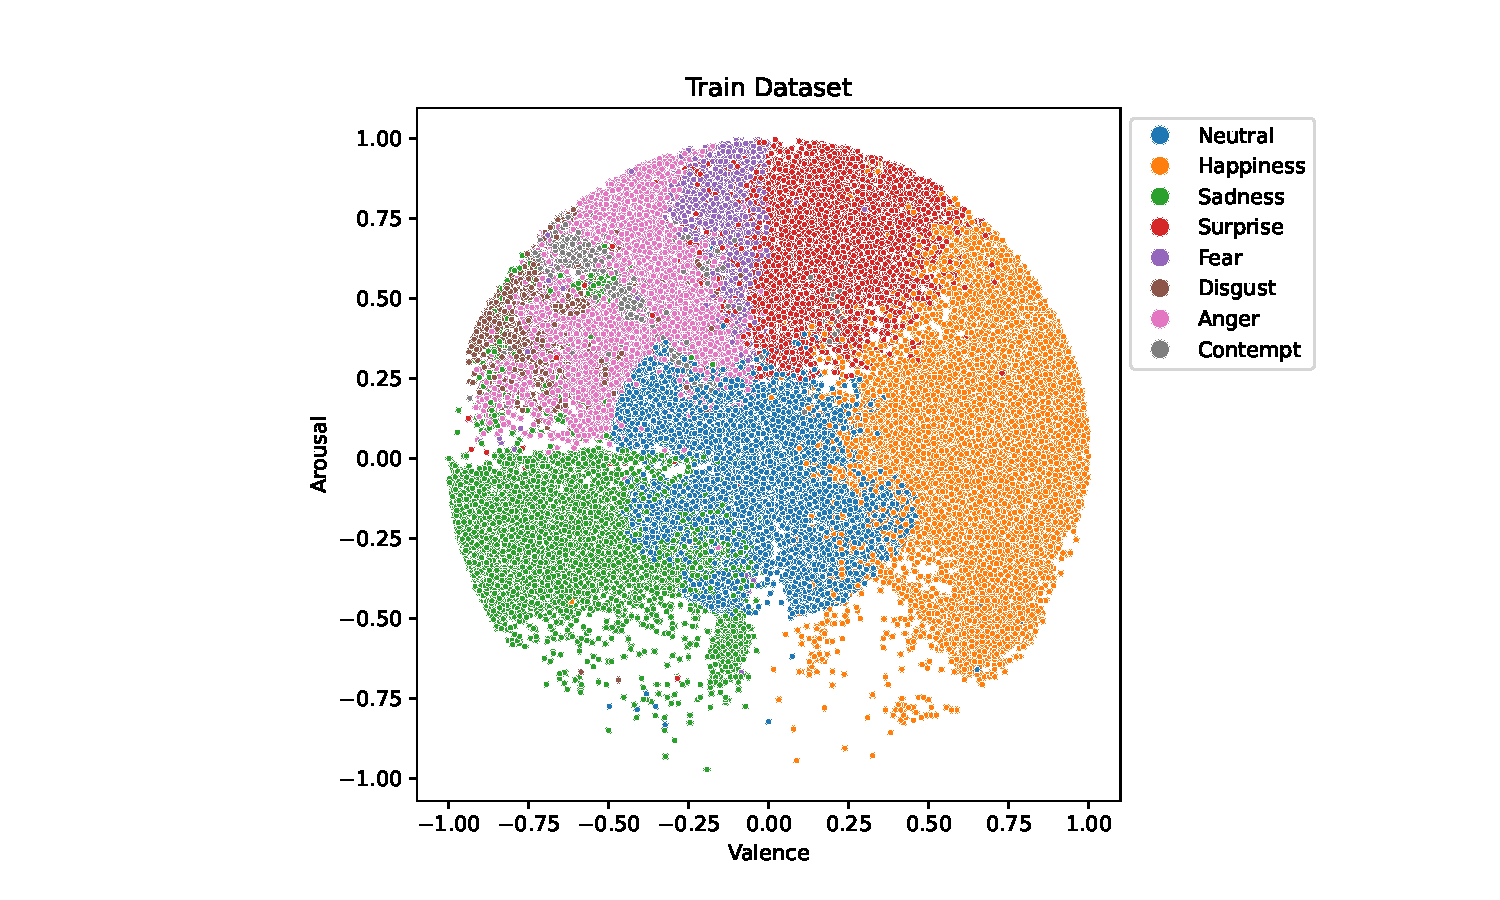
\includegraphics[scale = 0.15]{pictures/scatterplot.eps}
    \caption{Autonomous FZI shuttle}
    \label{fig:Scatterplot}
\end{figure}
\subsection{Emotic}

\newpage
\section{Train model}

\subsection{Improving the baseline AffectNet model}

\begin{center}
\begin{tabular}{c | c }
 Hyperparameter & Choosen \\ 
 \hline
 LR & \\
 \hline
\end{tabular}
\end{center}

compare only train classifier, only val and aro, both, and the recursive way. F1, Precision, Recall, RMSE, MSE, MAE

\begin{center}
\rotatebox{90}{
\begin{tabular}{c | c c c c c c}
 Approach & Precision & Recall & F1-Score & MSE & MAE & RMSE \\ 
 \hline
 Classifier & & & & & & \\
 \hline
 Val \& Aro & & & & & & \\
 \hline
 Combined & & & & & & \\
 \hline
 Preknowledge & & & & & & \\
 \hline
 Two models & & & & & & \\
 \hline
\end{tabular}
}
\end{center}

\newpage
\bibliographystyle{IEEEtran}  % Choose the IEEEtran bibliography style
\bibliography{literature.bib}  % Specify the name of your .bib file without the extension



\end{document}
